\documentclass[12pt, oneside]{article}

\usepackage[letterpaper, scale=0.8, centering]{geometry}
\usepackage{fancyhdr}
\setlength{\parindent}{0em}
\setlength{\parskip}{1em}

\pagestyle{fancy}
\fancyhf{}
\renewcommand{\headrulewidth}{0pt}
\rfoot{{\footnotesize Copyright Mia Minnes, 2024, Version \today~(\thepage)}}

\usepackage{titlesec}

\author{CSE105W24}

\newcommand{\instructions}{{\bf For all HW assignments:} Weekly homework 
may be done individually or in groups of up to 3 students. 
You may switch HW partners for different HW assignments. 
Please ensure your name(s) and PID(s) are clearly visible on the first page of your homework submission 
and then upload the PDF to Gradescope. If working in a group, submit only one submission per group: 
one partner uploads the submission through their Gradescope account and then adds the other group member(s) 
to the Gradescope submission by selecting their name(s) in the ``Add Group Members" dialog box. 
You will need to re-add your group member(s) every time you resubmit a new version of your assignment.
 Each homework question will be graded either for correctness (including clear and precise explanations and 
 justifications of all answers) or fair effort completeness. 
 For ``graded for correctness''
 questions: collaboration is allowed only with CSE 105 students in your group; 
 if your group has questions about a problem, you may ask in drop-in 
 help hours or post a private post (visible only to the Instructors) on Piazza.
 For ``graded for completeness''
 questions: collaboration is allowed with any CSE 105 students this quarter; 
 if your group has questions about a problem, you may ask in drop-in 
 help hours or post a public post on Piazza.

All submitted homework for this class must be typed. 
You can use a word processing editor if you like (Microsoft Word, Open Office, Notepad, Vim, Google Docs, etc.) 
but you might find it useful to take this opportunity to learn LaTeX. 
LaTeX is a markup language used widely in computer science and mathematics. 
The homework assignments are typed using LaTeX and you can use the source files 
as templates for typesetting your solutions.
To generate state diagrams of machines, we recommend using Flap.js
or JFLAP. Photographs of clearly hand-drawn diagrams may also be used. We recommend that you
submit early drafts to Gradescope so that in case of any technical difficulties, at least some of your
work is present. You may update your submission as many times as you'd like up to the deadline.


{\bf Integrity reminders}
\begin{itemize}
\item Problems should be solved together, not divided up between the partners. The homework is
designed to give you practice with the main concepts and techniques of the course, 
while getting to know and learn from your classmates.
\item You may not collaborate on homework questions graded for correctness with anyone other than your group members.
You may ask questions about the homework in office hours (of the instructor, TAs, and/or tutors) and 
on Piazza (as private notes viewable only to the Instructors).  
You \emph{cannot} use any online resources about the course content other than the class material 
from this quarter -- this is primarily to ensure that we all use consistent notation and
definitions (aligned with the textbook) and also to protect the learning experience you will have when
the `aha' moments of solving the problem authentically happen.
\item Do not share written solutions or partial solutions for homework with 
other students in the class who are not in your group. Doing so would dilute their learning 
experience and detract from their success in the class.
\end{itemize}

}

\newcommand{\gradeCorrect}{({\it Graded for correctness}) }
\newcommand{\gradeCorrectFirst}{\gradeCorrect\footnote{This means your solution 
will be evaluated not only on the correctness of your answers, but on your ability
to present your ideas clearly and logically. You should explain how you 
arrived at your conclusions, using
mathematically sound reasoning. Whether you use formal proof techniques or 
write a more informal argument
for why something is true, your answers should always be well-supported. 
Your goal should be to convince the
reader that your results and methods are sound.} }
\newcommand{\gradeComplete}{({\it Graded for completeness}) }
\newcommand{\gradeCompleteFirst}{\gradeComplete\footnote{This means you will 
get full credit so long as your submission demonstrates honest effort to 
answer the question. You will not be penalized for incorrect answers. 
To demonstrate your honest effort in answering the question, we 
expect you to include your attempt to answer *each* part of the question. 
If you get stuck with your attempt, you can still demonstrate 
your effort by explaining where you got stuck and what 
you did to try to get unstuck.} }

\usepackage{tikz}
\usetikzlibrary{automata,positioning,arrows}

\usepackage{amssymb,amsmath,pifont,amsfonts,comment,enumerate,enumitem}
\usepackage{currfile,xstring,hyperref,tabularx,graphicx,wasysym}
\usepackage[labelformat=empty]{caption}
\usepackage{xcolor}
\usepackage{multicol,multirow,array,listings,tabularx,lastpage,textcomp,booktabs}

% NOTE(joe): This environment is credit @pnpo (https://tex.stackexchange.com/a/218450)
\lstnewenvironment{algorithm}[1][] %defines the algorithm listing environment
{   
    \lstset{ %this is the stype
        mathescape=true,
        frame=tB,
        numbers=left, 
        numberstyle=\tiny,
        basicstyle=\rmfamily\scriptsize, 
        keywordstyle=\color{black}\bfseries,
        keywords={,procedure, div, for, to, input, output, return, datatype, function, in, if, else, foreach, while, begin, end, }
        numbers=left,
        xleftmargin=.04\textwidth,
        #1
    }
}
{}

\newcommand\abs[1]{\lvert~#1~\rvert}
\newcommand{\st}{\mid}

\newcommand{\cmark}{\ding{51}}
\newcommand{\xmark}{\ding{55}}


\newcommand{\SUBSTRING}{\textsc{Substring}}
\newcommand{\REP}{\textsc{Rep}}
\newcommand{\blank}{\scalebox{1.5}{\textvisiblespace}}


\title{HW1 : Regular Expressions and Deterministic Finite Automata}
\date{Due: : 4/7/22 at 5pm (no penalty late submission until 8am next morning), via Gradescope}


\begin{document}
\maketitle
\thispagestyle{fancy}


{\bf In this assignment,}

You will practice reading and
applying the definitions of alphabets, strings, languages, Kleene star, and regular expressions.
You will use regular expressions and relate them to languages and automata.
You will use precise notation to formally define the state diagram of DFA,
and you will use clear English to describe computations of DFA informally.


{\bf Resources}: To review the topics you are working with 
for this assignment, see the class material from Week 1.
We will post frequently asked questions and our answers to them in a 
pinned Piazza post.

{\bf Reading and extra practice problems}: Sipser Section 0, 1.3, 1.1.
Chapter 1 exercises 1.1, 1.2, 1.3, 1.18, 1.23.

\instructions

You will submit this assignment via Gradescope
(\href{https://www.gradescope.com}{https://www.gradescope.com}) 
in the assignment called ``HW1CSE105Sp22''.



{\bf Assigned questions}

\begin{enumerate}
\item ({\it Graded for correctness}\footnote{This means your solution will be
evaluated not only on the correctness of your answers, but on your ability to 
present your ideas clearly and logically. You should explain how you arrived at 
your conclusions, using 
mathematically sound reasoning. Whether you use formal proof techniques or 
write a more informal argument for why 
something is true, your answers should always be well-supported. Your goal 
should be to convince the reader that 
your results and methods are sound.}) 
For $L$ a set of strings over the alphabet $\{0,1\}$, we can define the following associated sets
\[
LZ(L) = \{ 0^k w \mid w \in L, k \in \mathbb{Z}, k \geq 0 \}
\]
\[
TZ(L) = \{ w 0^k \mid w \in L, k \in \mathbb{Z}, k \geq 0 \}
\]

Note: the commas in the set-builder definition indicate ``and''.

Note: $0^k$ is the result of concatenating $0$ with itself $k$ times; it is the string of $k$ $0$s.

Note: Formally, $LZ$ and $TZ$ are each functions, with domain the set of languages over $\{0,1\}$ and with codomain 
the set of languages over $\{0,1\}$.

\begin{enumerate}
\item Specify an example language $L_1$ over $\{0,1\}$ where $LZ(L_1) = \Sigma^*$, or explain why there is no such 
example. A complete solution will include either (1) a precise and clear 
description of your example language $L_1$ and a precise and clear description of the result of computing $LZ(L_1)$
using the definitions to justify this description and justifying the set equality with $\Sigma^*$, or (2) a sufficiently
general and correct argument why there is no such example, referring back to the relevant definitions.
\item Specify an example language $L_2$ over $\{0,1\}$ where $LZ(L_2)$ is a finite set, or explain why there is no such 
example. A complete solution will include either (1) a precise and clear 
description of your example language $L_2$ and a precise and clear description of the result of computing $LZ(L_2)$
using the definitions to justify this description and justifying why it is finite, or (2) a sufficiently
general and correct argument why there is no such example, referring back to the relevant definitions.
\item Specify an example language $L_3$ over $\{0,1\}$ where $LZ(L_3) = TZ(L_3)$, or explain why there is no such 
example. A complete solution will include either (1) a precise and clear 
description of your example language $L_3$ and a precise and clear description of the results of computing $LZ(L_3)$
and $TZ(L_3)$ using the definitions to justify this description and justifying the set equality, or (2) a sufficiently
general and correct argument why there is no such example, referring back to the relevant definitions.
\end{enumerate}

\item ({\it Graded for correctness})
Consider the two regular expressions over $\Sigma = \{ 0, 1 \}$
\[
R_1 = (~(000 \cup 111)^* ~\cup~ (01)^*~)
\qquad \qquad
R_2 = (~(000)^*(111)^* (\varepsilon \cup 0\cup1))
\]
You will prove that 
\[
L(R_1) \not \subseteq L(R_2) ~ \text{and} ~ L(R_2) \not \subseteq L(R_1)  
~ \text{and} ~ L(R_1) \cap L(R_2)  \neq \emptyset
~ \text{and} ~ L(R_1) \cup L(R_2)  \neq \Sigma^*
\]
by giving four example strings that witness these properties.
\begin{enumerate}
\item Specify an example string $w_1$ such that $w_1 \in L(R_1) \cap L(R_2)$.
 Briefly justify your choice, referring to the definitions of the regular expressions and their semantics.
\item Specify an example string $w_2$ such that $w_2 \in L(R_1) \cap \overline{L(R_2)}$.
Briefly justify your choice, referring to the definitions of the regular expressions and their semantics.
\item Specify an example string $w_3$ such that $w_3 \in \overline{L(R_1)} \cap L(R_2)$.
Briefly justify your choice, referring to the definitions of the regular expressions and their semantics.
\item Specify an example string $w_4$ such that $w_4 \in \overline{L(R_1)} \cap \overline{L(R_2)}$.
Briefly justify your choice, referring to the definitions of the regular expressions and their semantics.
\end{enumerate}


\item  ({\it Graded for fair effort completeness}\footnote{This means 
you will get full credit so long as your submission demonstrates honest 
effort to answer the question. You will not be penalized for incorrect answers. 
To demonstrate your honest effort in answering the question, we ask that you 
include your attempt to answer *each* part of the question. If you get stuck 
with your attempt, you can still demonstrate your effort by explaining where 
you got stuck and what you did to try to get unstuck. }) 
\begin{enumerate}
\item Pick a four letter alphabet (a nonempty finite set), and specify it, e.g.\ by filling in the blank 
$\Sigma =  \underline{\text{fill in your alphabet here}}$.

Then, pick a language of cardinality (size) $2$ over this alphabet, and specify it, e.g.\ by filling in the blank
\[
L =  \underline{\text{fill in your language here}}
\]
{\it Note: we encourage you to pay attention to syntax here.  There are many correct answers; please be 
precise in how you present the sets you choose.}

\item Give a regular expression that describes the language $L$ you defined in part (a).  
Briefly justify why your regular expression
works.
\item Give a DFA that recognizes your language $L$ you defined in part (a).  
Specify your DFA {\bf both} using a formal definition
{\bf and} a state diagram. Briefly justify why your DFA works.
\end{enumerate}

\item ({\it Graded for correctness}) Consider the DFA $C$ given by the state diagram below.
\begin{figure}[h]
   \centering
   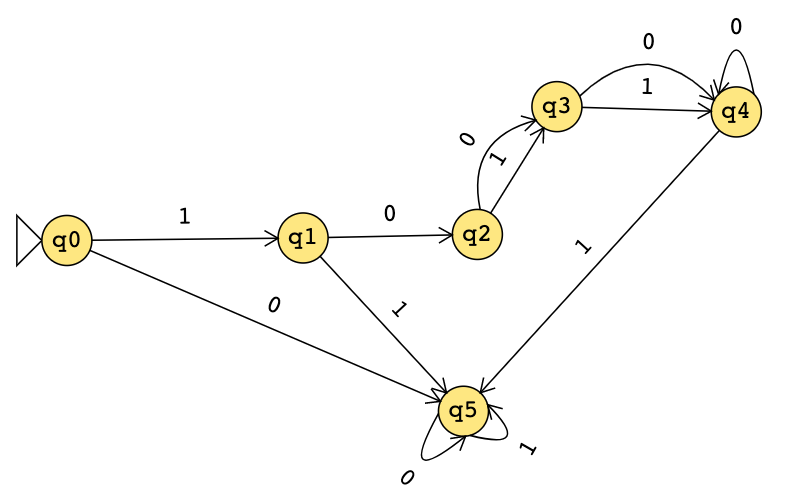
\includegraphics[width=3in]{../../resources/machines/hw1dfaCSE105Sp22.png}
   \caption{State diagram for DFA $C$}
\end{figure}

Suppose someone tells you that the formal definition of this DFA is 
\[
(Q, \Sigma, \delta, q_0, F) =  (\{ q0, q1, q2, q3, q4, q5 \}, \{0,1,2\}, \delta, q0, q0)
\]
where $\delta: Q \times \Sigma \to Q$ is given by 
\[
\hspace{-1in}\delta ( (q, 0) ) = \begin{cases}
q5 & \text{if $q=q0$} \\
qj & \text{if $q=qi$ and $i \in \{1,2,3\}$ and $j=i+1$} \\
q & \text{if $q \in \{q4,q5\}$} \\
\end{cases}  \qquad \delta ( (q, 1) ) = \begin{cases}
    q1 & \text{if $q=q0$} \\
    q5 & \text{if $q \in \{q1,q4,q5\}$} \\
    \delta( (q,0) ) & \text{if $q=q2$ or $q=q3$} \\
    \end{cases}
\]
\begin{enumerate}
\item Confirm that this formal description is correct (in that it is consistent with the 
state diagram), or fix any and all mistakes in it.
In your solution, explicitly address whether the description of the set of states is correct, whether the 
description of the alphabet is correct, 
whether the description of the transition function is correct, 
whether the description of the start state is correct, and whether 
the description of the accept states is correct, and why.

\item Modify the set of accept states of this state diagram to get a different DFA 
(with the same set of states, alphabet, start state, and transition function) 
that recognizes an infinite language. Your solution should include the 
diagram of this new DFA and an explanation of why the language it recognizes
is infinite.
\end{enumerate}


\item ({\it Graded for fair effort completeness})
Which of the following are valid descriptions using the terminology we have used in 
class and in the book so far? For those that aren't, explain what's wrong. For those that are, 
give an example of what's being described.
\begin{enumerate}
\item A finite automaton accepts a regular expression.
\item The language described by a regular expression is a finite automaton.
\item The empty string is the language of some regular expression.
\item A string of length one uses one symbol from the alphabet.
\item The input string runs a finite automaton.
\end{enumerate}


\end{enumerate}
\end{document}